\section{Auswertung}
\label{sec:Auswertung}

\subsection{Vermessung von Fehlstellen im Acrylblock}
\label{sec:fehlstelle}
Der zu vermessende Acrylblock mit 11 Fehlstellen hat eine Höhe von $h_{Block} = 8.03 cm$.
Dieser wurde mit einer Schieblehre vermessen.
Beim A-Scan im Impuls-Echo-Verfahren mit der 2 MHz Sonde sind für die Fehlstellen die Laufzeiten $\Delta t_{oben}$ und $\Delta t_{unten}$, jeweils von der Ober- und Unterseite des Blocks vermessen, in Tabelle \ref{tab:tab1} aufgetragen.
\begin{table}
  \centering
  \caption{Messwerte Fehlstellen.}
  \label{tab:tab1}
\begin{tabular}{c c c c c}
  \toprule
  Fehlstelle & $\Delta t_{oben}$ in $\mu$s & $\Delta t_{unten}$ in $\mu$s & $s_{oben}$ in mm & $s_{unten}$ in mm\\
  \midrule
  1  &  44.6  &  9.6  &  61.0  &  13.0  \\
  2  &  39.1  &  15.8  &  54.0  &  22.0  \\
  3  &  33.8  &  21.9  &  47.0  &  30.0  \\
  4  &  28.2  &  28.1  &  39.0  &  39.0  \\
  5  &  22.4  &  34.1  &  31.0  &  47.0  \\
  6  &  16.7  &  39.9  &  23.0  &  55.0  \\
  7  &  10.8  &  45.7  &  15.0  &  63.0  \\
  8  &  4.9  &  51.5  &  7.0  &  71.0  \\
  9  &  40.4  &  11.0  &  55.0  &  15.0  \\
  10  &  12.8  &  44.8  &  18.0  &  61.0  \\
  11  &  14.1  &  43.6  &  19.5  &  59.0  \\
  \bottomrule
\end{tabular}
\end{table}
\FloatBarrier
Die Strecken $s_{oben}$ und $s_{unten}$ sind der Abstand der Fehlstellen zum oberen und unteren Rand des Acrylblocks, mit einer Schieblehre vermessen.
Aus der Laufzeit, der Schallgeschwindigkeit in Acryl mit $c_{Ac} = 2730 \frac{m}{s}$ \cite{schall} und der Formel
\begin{equation}
  d_{oben} = c_{Ac} \cdot \frac{\Delta t_{oben}}{2}
  \label{eqn:glA1}
\end{equation}
werden die Abstände nach oben und (analog zur Gleichung \ref{eqn:glA1}) unten zum Acrylblock errechnet.
Aus diesen Werten kann dann durch die Gleichung \ref{eqn:glA2}
\begin{equation}
  d = h_{Block} - d_{oben} - d_{unten}
  \label{eqn:glA2}
\end{equation}
der Durchmesser der Fehlstellen bestimmt werden.
Die Abstände und daraus resultierenden Durchmesser sind in Tabelle \ref{tab:tab2} eingetragen.
Die Größe $d_{Messung}$ ist der Messwert des Durchmessers. 
Er wurde mit $d_{Messung} = h - s_{oben} - s_{unten}$ berechnet.
\begin{table}
  \centering
  \caption{Durchmesser der Fehlstellen.}
  \label{tab:tab2}
\begin{tabular}{c c c c c c}
  \toprule
  Fehlstelle & $d_{oben}$ in mm & $d_{unten}$ in mm & $d$ in mm & $d_{Messung}$ in mm & Abweichung in \%\\
  \midrule
  1  &  60.879  &  13.104 & 6.317 & 6.3 & 0.27  \\
  2  &  53.3715  &  21.567 & 5.3615 & 4.3 & 24.69  \\
  3  &  46.137  &  29.8935 & 4.2695 & 3.3 & 29.38  \\
  4  &  38.493  &  38.3565 & 3.4505 & 2.3 & 50.02  \\
  5  &  30.576  &  46.5465 & 3.1775 & 2.3 & 38.15  \\
  6  &  22.7955  &  54.4635 & 3.041 & 2.3 & 32.22  \\
  7  &  14.742  &  62.3805 & 3.1775 & 2.3 & 38.15  \\
  8  &  6.6885  &  70.2975 & 3.314 & 2.3 & 44.09  \\
  9  &  55.146  &  15.015 & 10.139 & 10.3 & 1.56  \\
  10  &  17.472  &  61.152 & 1.676 & 1.3 & 28.92  \\
  11  &  19.2465  &  59.514 & 1.5395 & 1.8 & 14.47  \\
  \bottomrule
\end{tabular}
\end{table}
\FloatBarrier

\subsection{Auflösungsvermögen}
\label{sec:auf}
Bei den zwei sehr nah beieinander liegenden Fehlstellen 10 und 11 wird das Auflösungsvermögen verschiedener Sonden untersucht.
Es wurde ein A-Scan mit einer 1 MHz und einer mit einer 4 MHz Sonde durchgeführt.
Die Ergebnisse sind in den Abbildungen \ref{fig:abbA1} und \ref{fig:abbA2} zu sehen.

\begin{figure}
  \centering
  \includegraphics{data/doppel1MHz.jpg}
  \caption{Auflösungsvermögen der 1 MHz Sonde.}
  \label{fig:abbA1}
\end{figure}
\FloatBarrier

\begin{figure}
  \centering
  \includegraphics{data/doppel4MHz.jpg}
  \caption{Auflösungsvermögen der 4 MHz Sonde.}
  \label{fig:abbA2}
\end{figure}
\FloatBarrier

Es ist klar erkennbar, dass die 4 MHz Sonde ein wesentliches besseres Auflösungsvermögen besitzt, aber dafür schneller an seiner Amplitudenstärke verliert.
Hingegen besitzt die 1 MHz Sonde einen hoheren Ausschlag, aber bei schlechterem Auflösungsvermögen.
%In Diskussion Frequenzabhängigkeit der Auflösung und Eindringtiefe

\subsection{B-Scan des Acrylblocks}
\label{sec:bscan}

\begin{figure}
  \centering
  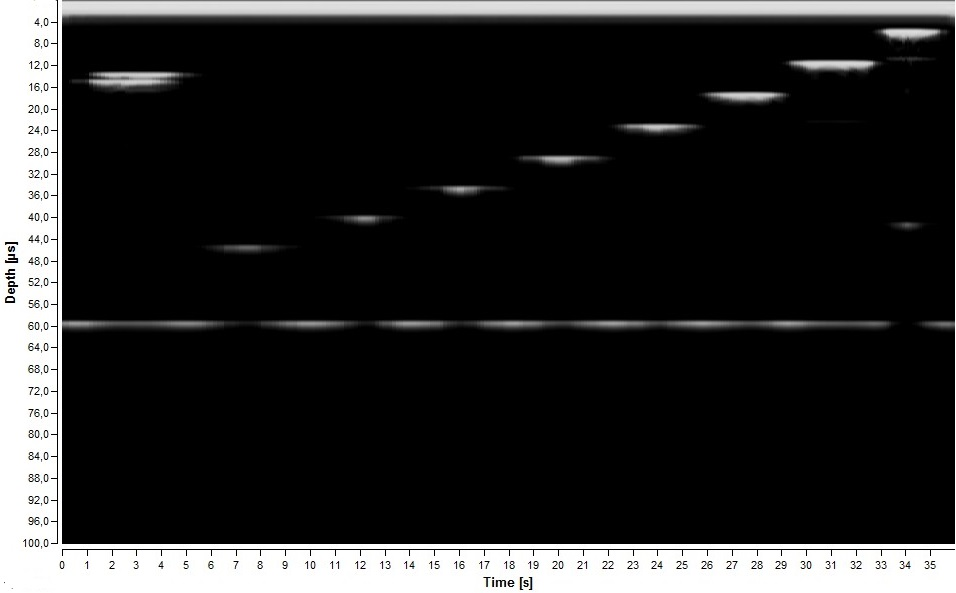
\includegraphics[width = 10cm]{data/BScanOben.jpg}
  \caption{B-Scan von oben.}
  \label{fig:abbA3}
\end{figure}
\FloatBarrier

\begin{figure}
  \centering
  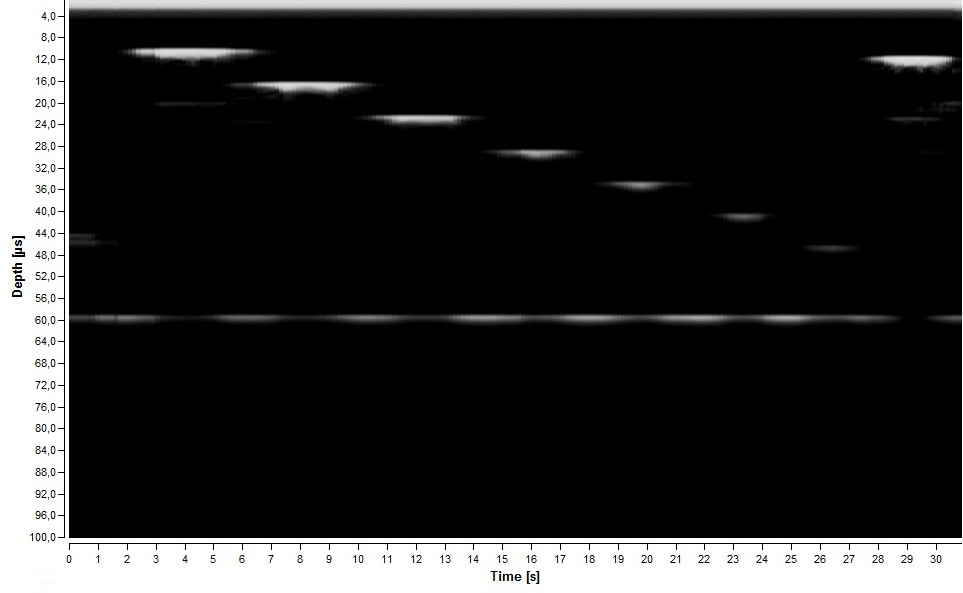
\includegraphics[width = 10cm]{data/BScanUnten.jpg}
  \caption{B-Scan von unten.}
  \label{fig:abbA4}
\end{figure}
\FloatBarrier

Die beiden B-Scans in Abbildung \ref{fig:abbA3} und \ref{fig:abbA4} wurden mit der 2 MHz Sonde durchgeführt und zeigen ein gutes Bild des Acrylblocks mit seinen Fehlstellen.
Aber die tiefer im BLock liegenden Stellen werden schlecht bis garnicht dargestellt. 
Somit ist es ein nur unvollständiges Bild des Acrylblocks.
Auch die zwei kleinen und sehr nah beieinander liegenden Fehlstellen 10 und 11 sind in Abbildung \ref{fig:abbA3} zu erkennen, obwohl sie sich doch überschneiden.
Der unterste fast durchgezogene weiße Strich ist jeweils der Boden des Acrylblocks.

\subsection{TM-Scan eines Herzmodels}
\label{sec:herz}

\begin{figure}
  \centering
  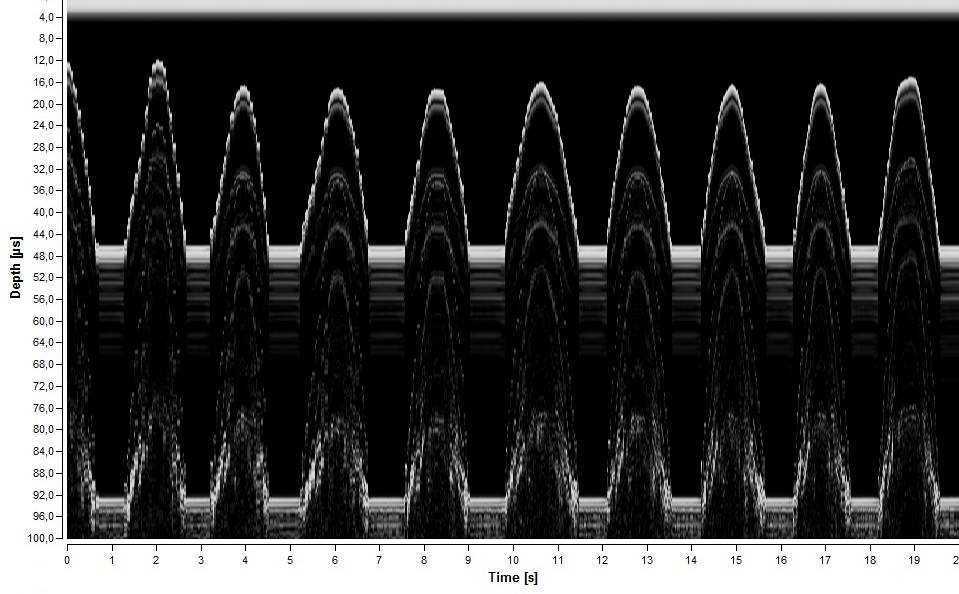
\includegraphics[width = 10cm]{data/TMScan.jpg}
  \caption{TM-Scan des Herzmodels.}
  \label{fig:abbA5}
\end{figure}
\FloatBarrier

Aus der Abbildung \ref{fig:abbA5} ist die Herzfrequenz abzulesen.
Es werden $P = 10$ Peaks auf $t_P = 19$s gezählt, womit sich die Frequenz zu
\begin{align*}
  \nu = \frac{P-1}{t_P} = \frac{9}{19} = 0.474 \text{Hz} 
\end{align*}
berechnen lässt.
Mit dem gemessenen Radius $r = 22.7$ mm des Herzens und der Vermessung mit A-Scan im Ruhe Zustand und im aufgepumpten Zustand wird das enddiastolische ($EDV$) und das endsystolische Volumen ($ESV$) mit
\begin{equation}
  V = c_{Wasser} \frac{\Delta t}{2} \cdot \pi r^2
  \label{eqn:glA3}
\end{equation} 
berechnet.
Für die Schallgeschwindigkeit in Wasser wurde der Literaturwert von $c_{Wasser} = 1480 \frac{m}{s}$ \cite{schall} gewählt.
Aus dem A-Scan für beide Volumen wurden $\Delta t_{EDV} = 45.8 \mu $s und $\Delta t_{ESV} = 23.9 \mu$s abgelesen.
Für das $EDV$ ergibt sich mit Gleichung \ref{eqn:glA3} $EDV = 5.47 \cdot 10^{-5}$ mm$^3$ und für das $ESV$ ergibt sich $ESV = 28.6 \cdot 10^{-5}$ mm$^3$.
Aus diesen beiden Werten und der Frequenz wird das Herzvolumen wie folgt berechnet:
\begin{equation}
  HZV = (EDV - ESV) \cdot \nu
  \label{eqn:glA4}
\end{equation}
Mit Gleichung \ref{eqn:glA4} und den vorangegangenen Werten wird $HZV =  1.24 \cdot 10^{-5}$ mm$^3$ berechnet.
Dies ist das Schlagvolumen des Herzens.